\section{\Large{Лекция 2}}
Будем исследовать ОДУ, заданное в форме Коши:
\begin{equation} \label{eq:def_DY_Koshi}
y'(x) = f(x, y(x))
\end{equation}
$x$ принадлежит некоторому промежутку (отрезку, интервалу, полуинтервалу с конечными или бесконечными границами) $I$, $y(x \in I): x \to D \subseteq \RR$. Здесь и далее будем обозначать $G = I \times D$.
\subsection{\large{Метод изоклин}}
\begin{Def} \fcolorbox{g}{g}{Изоклина}\\
\tit{Изоклина} (от линия постоянного наклона) -- ГМТ для \eqref{eq:def_DY_Koshi}, задаваемое в виде $f(x,y) = k, ~ k = const$
\end{Def}
Рассмотрим уравнение $y'(y+x) = (y-x)$\footnote{На лекции был пример $y'(x-y)=(x+y)$, в сущности ничем не отличающийся от приведенного здесь} 

\begin{wrapfigure}{l}{0.5\linewidth}
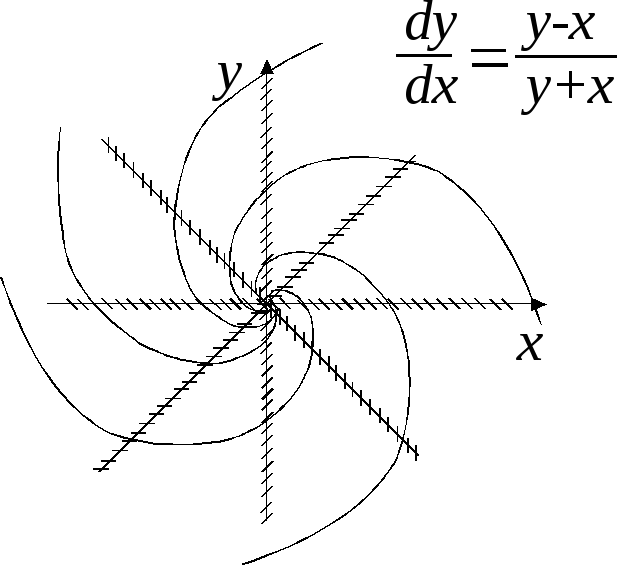
\includegraphics[width=\linewidth]{izoklina.png}
\caption{}  \label{pic_izoklina}
\end{wrapfigure}
Построим его изоклины. Для этого будем фиксировать значения $y' = k$ :
\begin{enumerate}
\item $k = 0$: $y = x$
\item $k = 1$: $x = 0$
\item $k = -1$: $y = 0$
\item $k \rar +\INF$: $y = -x$
\end{enumerate}
Построим прямые 1--4, при пересечении этих прямых, касательная интегральной кривой, должна иметь наклон, соответствующий $k$, если точнее $k$ -- значения $\tg \al$, где $\al$ -- угол между касательной и $OX$. Затем можно графически строить некоторые интегральные кривые см. рис. \ref{pic_izoklina}.
\clearpage
\subsection{\large{Задача Коши}}
\begin{Def} \fcolorbox{g}{g}{Расширенное понятие интегральной кривой} \\
кривая
\begin{equation}
    \Ga = \left\{ \begin{aligned}
x &= \psi(t) \\
y &= \phi(t)
\end{aligned} \right., ~~t \in I_t
\end{equation}
называется интегральной кривой ОДУ $y' = f(x, y)$ если: 
\begin{itemize}
    \item $\pair{ \psi(t)}{ \phi(t) } \in G, ~ \forall t \in I_t$
    \item $\psi(t) \in C(I_t), ~\phi(t) \in C(I_t)$
    \item  $\psi'(t)^2 + \phi'(t)^2 \neq 0, \forall t \in I_t$
    \item $\phi'(t) = f(\phi(t), \psi(t)) \psi'(t)$
\end{itemize}
\end{Def}
\begin{Def} \fcolorbox{g}{g}{Задача Коши}\\
Задача Коши состоит в том, что бы для заданного ДУ среди множества всех решений, найти интегральную кривую, удовлетворяющую начальным данным, заданным в виде точек, через которые эта интегральная кривая должна приходить
\end{Def}
\begin{example}
рассмотрим ОДУ : $ \br{e^x+1}^2 + \br{e^{2x}-1}y = 0$, так же зададим начальные условия: $y(0) = 1 / 4$ (получили задачу Коши).\\
Общее решение:
\begin{equation}
    y = C \frac{e^x}{ \br{e^x+1}^2}, ~ C = const
\end{equation}
Из начальных условий определим константу С:
\begin{equation}
    \frac{1}{4} = C \frac{e^0}{ \br{e^0+1}^2} \rar  C = 1
\end{equation}
\end{example}
\subsubsection{Теорема о существовании и единственности решения з. Коши}
\begin{theorem} \label{th:exists_and_one_solutin_task_Koshi} \fcolorbox{o}{o}{Существование и единственность решения задачи Коши} \\
Пусть дана задача Коши:  $y' = f(x, y), ~ y(x_0) = y_0$ 
\begin{enumerate}
    \item $f(x, y) \in C(G)$, то тогда решение задачи существует $\forall \pair{x_0}{y_0} \in G$
    \item $\frac{df}{dy} \in C(G)$ и выполняется пункт (1), то существует такая окрестность $x_0$ : $U_{\de}(x_0) \subseteq I$, что решение в ней единственно
\end{enumerate}
\end{theorem}
Теорема \ref{th:exists_and_one_solutin_task_Koshi} будет доказана позже в курсе (ориентировочно в конце этого семестра, под Новый год)
\begin{example}
Задача Коши: $y' = 3 y^{2/3}, y(2) = 1$\\
$f(x,y) = y^{2/3}$ -- непрерывна, значит решение существует\\
$f'_{y} = 2 y^{-1/3}$ -- непрерывна при $y \neq 0$, таким образом к некоторой окрестности $x=2$ решение единственно. Но! Покажем, что ошибочно полгать, что теорема \ref{th:exists_and_one_solutin_task_Koshi} имеет глобальный характер.\\
Разделив переменные в ДУ и опредлив константу интегрирования, получаем что $y(x) \hm{=} (x-1)^3$, которая удовлетворяет всем условия задачи.\\
Рассмотрим две другие функции:
\begin{align}
    \phi_1(x) =  \left\{ \begin{aligned}
     &0, ~ x < 1 \\
     &(x-1)^3, ~ x \geqslant 1
    \end{aligned} \right. && \phi_2 (x) = \left \{ \begin{aligned}
    & \br{x+1}^3, ~ x \leqslant 3 \\
    & 0, ~ -3 \leqslant x \leqslant 1 \\
    & \br{x-1}^3 , ~ x >1 
    \end{aligned} \right.
\end{align}
Легко проверить, что обе функции удовлетворяют задаче Коши, но не совпадают друг с другом.
\end{example}
\subsubsection{Теорема о продолжении решения}
\begin{Def} \fcolorbox{g}{g}{Точка неединственности} \\
Точка $(x_0, y_0)$ называется \tit{точкой неединственности} для заданного ДУ, если существуют две интегральные кривые $f(x), g(x)$ -- решения ДУ, проходящие через $(x_0, y_0)$ такие что:
\begin{itemize}
    \item $f'(x_0) = g'(x_0)$ (имеют общую касательную)
    \item $f(x)$ и $g(x)$ локально различны (не совпадают в любой окрестности $(x_0, y_0)$)
\end{itemize}
\end{Def}
\begin{Def} \fcolorbox{g}{g}{Особое решение} \\
Решение ДУ особое, если каждая его точка -- точка неединственности.
\end{Def}
Для дальнейшего изложения зафиксируем область определения $I$ ($x \in I$). Рассмотрим $I_1, I_2 : I_1 \subseteq I, I_2 \subseteq I, I^* = I_1 \cap I_2 \neq \varnothing$ \\
Пусть существуют две интегральных кривых -- решения ДУ: $y = \phi_1(x), x \in I_1 ,~ y = \phi_2(x), x \in I_2$, причем $x \in I^* \Rar \phi_1(x) = \phi_2(x)$\\.
\begin{Def} \fcolorbox{g}{g}{Продолжение решения} \\
В случае, если $I^* = I_1$, то $y = \phi_2(x)$ называется \tit{продолжением} решения $y = \phi_1(x)$
\end{Def}
\begin{note}
если $I^*$ -- точка, то термин продолжение заменяется на термин \tit{стыковка}
\end{note}
\begin{note}
Если $I^* \neq I_1 \land I^* \neq I_2$, то $y = \phi_1(x), y = \phi_2(x)$ являются продолжением одно другого, а
\begin{equation}
    y = \phi^*(x) = \left\{ \begin{aligned}
    & \phi_1(x), ~  x \in I_1 \\
    & \phi_2(x), ~ x \in I_2 \setminus I^*
 \end{aligned} \right.
 \end{equation}
 является решением на $I_1 \cup I_2$.
\end{note}
\begin{Def} \fcolorbox{g}{g}{Непродолжаемое решение} \\
решение $y = \phi(x)$ называется непродолжаемым, если не существует решения ДУ, являющимся его продолжением.
\end{Def}
\begin{example}
Рассмотрим
\begin{equation}
    \left\{ \begin{aligned} 
    &y' = -y^2 \\
    &y(1) = -1
    \end{aligned}    \right.
\end{equation}
это з. Коши, ДУ с разделяемыми переменными, разделив переменные и проинтегрировав получаем:
\begin{equation}
    y = \frac{1}{x+C}
\end{equation}
Из начальных условий $C=2$, окончательно получаем:
\begin{equation}
    y = \frac{1}{x-2}
\end{equation}
Построим график интегральной кривой при $x \in I = (- \INF ; 2)$. График этой функции имеет вертикальную асимптоту $x = 2$, по определению, если $f(x, y)$ решение ДУ то $f(x, y)$ непрерывна на области $G$, в данном случае из-за вертикальной асимптоты, решение не может быть продолженным вправо.
\end{example}
\begin{theorem} \label{th:continuation of the solution on a restricted area} \fcolorbox{o}{o}{ О продолжении решения на компакте} \\
пусть $G$ -- компакт, $f(x, y)$ -- решение ДУ на некотором подмножестве  $G$, причем $f(x, y) \in C(G),~  f'_y(x, y) \in C(G)$, то тогда $f(x,y)$ можно продолжить в обе стороны, до выхода его графика на границу области $G$.
\end{theorem}
Теорема \ref{th:continuation of the solution on a restricted area} так же будет доказана в к конце семестра, после доказательства теоремы \ref{th:exists_and_one_solutin_task_Koshi}